\section{687 --- Longest Univalue Path}
Given a binary tree, find the length of the longest path where each node in the path has the same value. This path may or may not pass through the root.

The length of path between two nodes is represented by the number of edges between them.

 

\paragraph{Example 1:}

\begin{flushleft}
\textbf{Input}:

\begin{figure}[H]
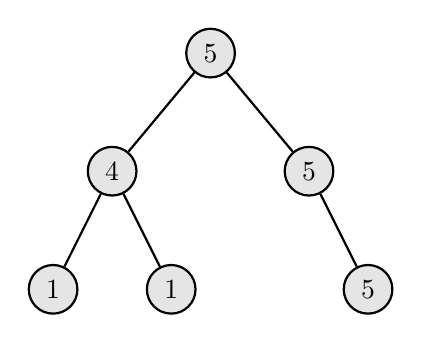
\begin{tikzpicture}
[every node/.style={draw, circle, fill=gray!20!, minimum size=5mm},
level 1/.style={sibling distance=25mm},
level 2/.style={sibling distance=15mm},
thick]
\node{5}
child{node{4} child{node{1}} child{node{1}} }
child{node{5} child[missing] child{node{5}}};
\end{tikzpicture}
\end{figure}

\textbf{Output}: 2

 
\end{flushleft}

\paragraph{Example 2:}

\begin{flushleft}
\textbf{Input}:

\begin{figure}[H]
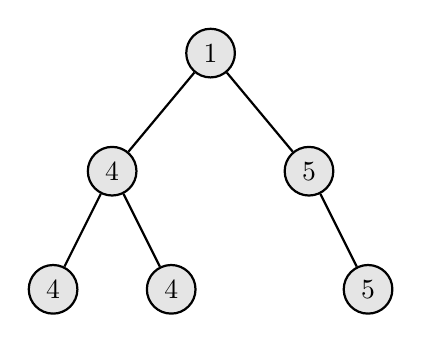
\begin{tikzpicture}
[every node/.style={draw, circle, fill=gray!20!, minimum size=5mm},
level 1/.style={sibling distance=25mm},
level 2/.style={sibling distance=15mm},
thick]
\node{1}
child{node{4} child{node{4}} child{node{4}} }
child{node{5} child[missing] child{node{5}}};
\end{tikzpicture}
\end{figure}


\textbf{Output}: 2
\end{flushleft}

 

\paragraph{Note: }
\begin{itemize}
\item The given binary tree has not more than 10000 nodes. The height of the tree is not more than 1000.
\end{itemize}

\subsection{Recursion}
Suppose $l$ and $r$ are the length of two longest path which are starting from current node's left and right child respectively.

Similar to the problem that finding the path sum of the tree, the recursive function will return the longest path that is from current node, and the length of the global longest path will be the parameter of the function.

When current node's value is equal to left child's value, we extend $l$ to $l+1$ because the path can extend to current node, otherwise set $l$ to 0.

Similarly, we extend $r$ to $r+1$ when right child and current node have same values, otherwise, set $r$ to 0.

Then, we update global maximum length as maximum of itself and ($l+r$).

\setcounter{lstlisting}{0}
\begin{lstlisting}[style=customc, caption={Recursion}]
int longestUnivaluePath( TreeNode* root )
{
    int ans = 0;

    dfs( root, ans );

    return ans;
}

int dfs( TreeNode* node, int& ans )
{
    if( !node )
    {
        return 0;
    }

    int left = dfs( node->left, ans );

    int from_left = 0;

    if( node->left )
    {
        if( node->left->val == node->val )
        {
            //extend left length
            from_left = left + 1;
        }
    }

    int right = dfs( node->right, ans );
    int from_right = 0;
    if( node->right )
    {
        if( node->right->val == node->val )
        {
            //extend right length
            from_right = right + 1;
        }
    }

    //return maximum of left and right
    int ret = ( max )( from_left, from_right );
    //update global maximum
    ans = ( max )( ans, from_left + from_right );

    return ret;
}
\end{lstlisting}